\documentclass{standalone}
\usepackage{tikz}
\usetikzlibrary{patterns, positioning}
\usepackage[sfdefault]{ClearSans} %% option 'sfdefault' activates Clear Sans as the default text font
\usepackage[T1]{fontenc}

\begin{document}
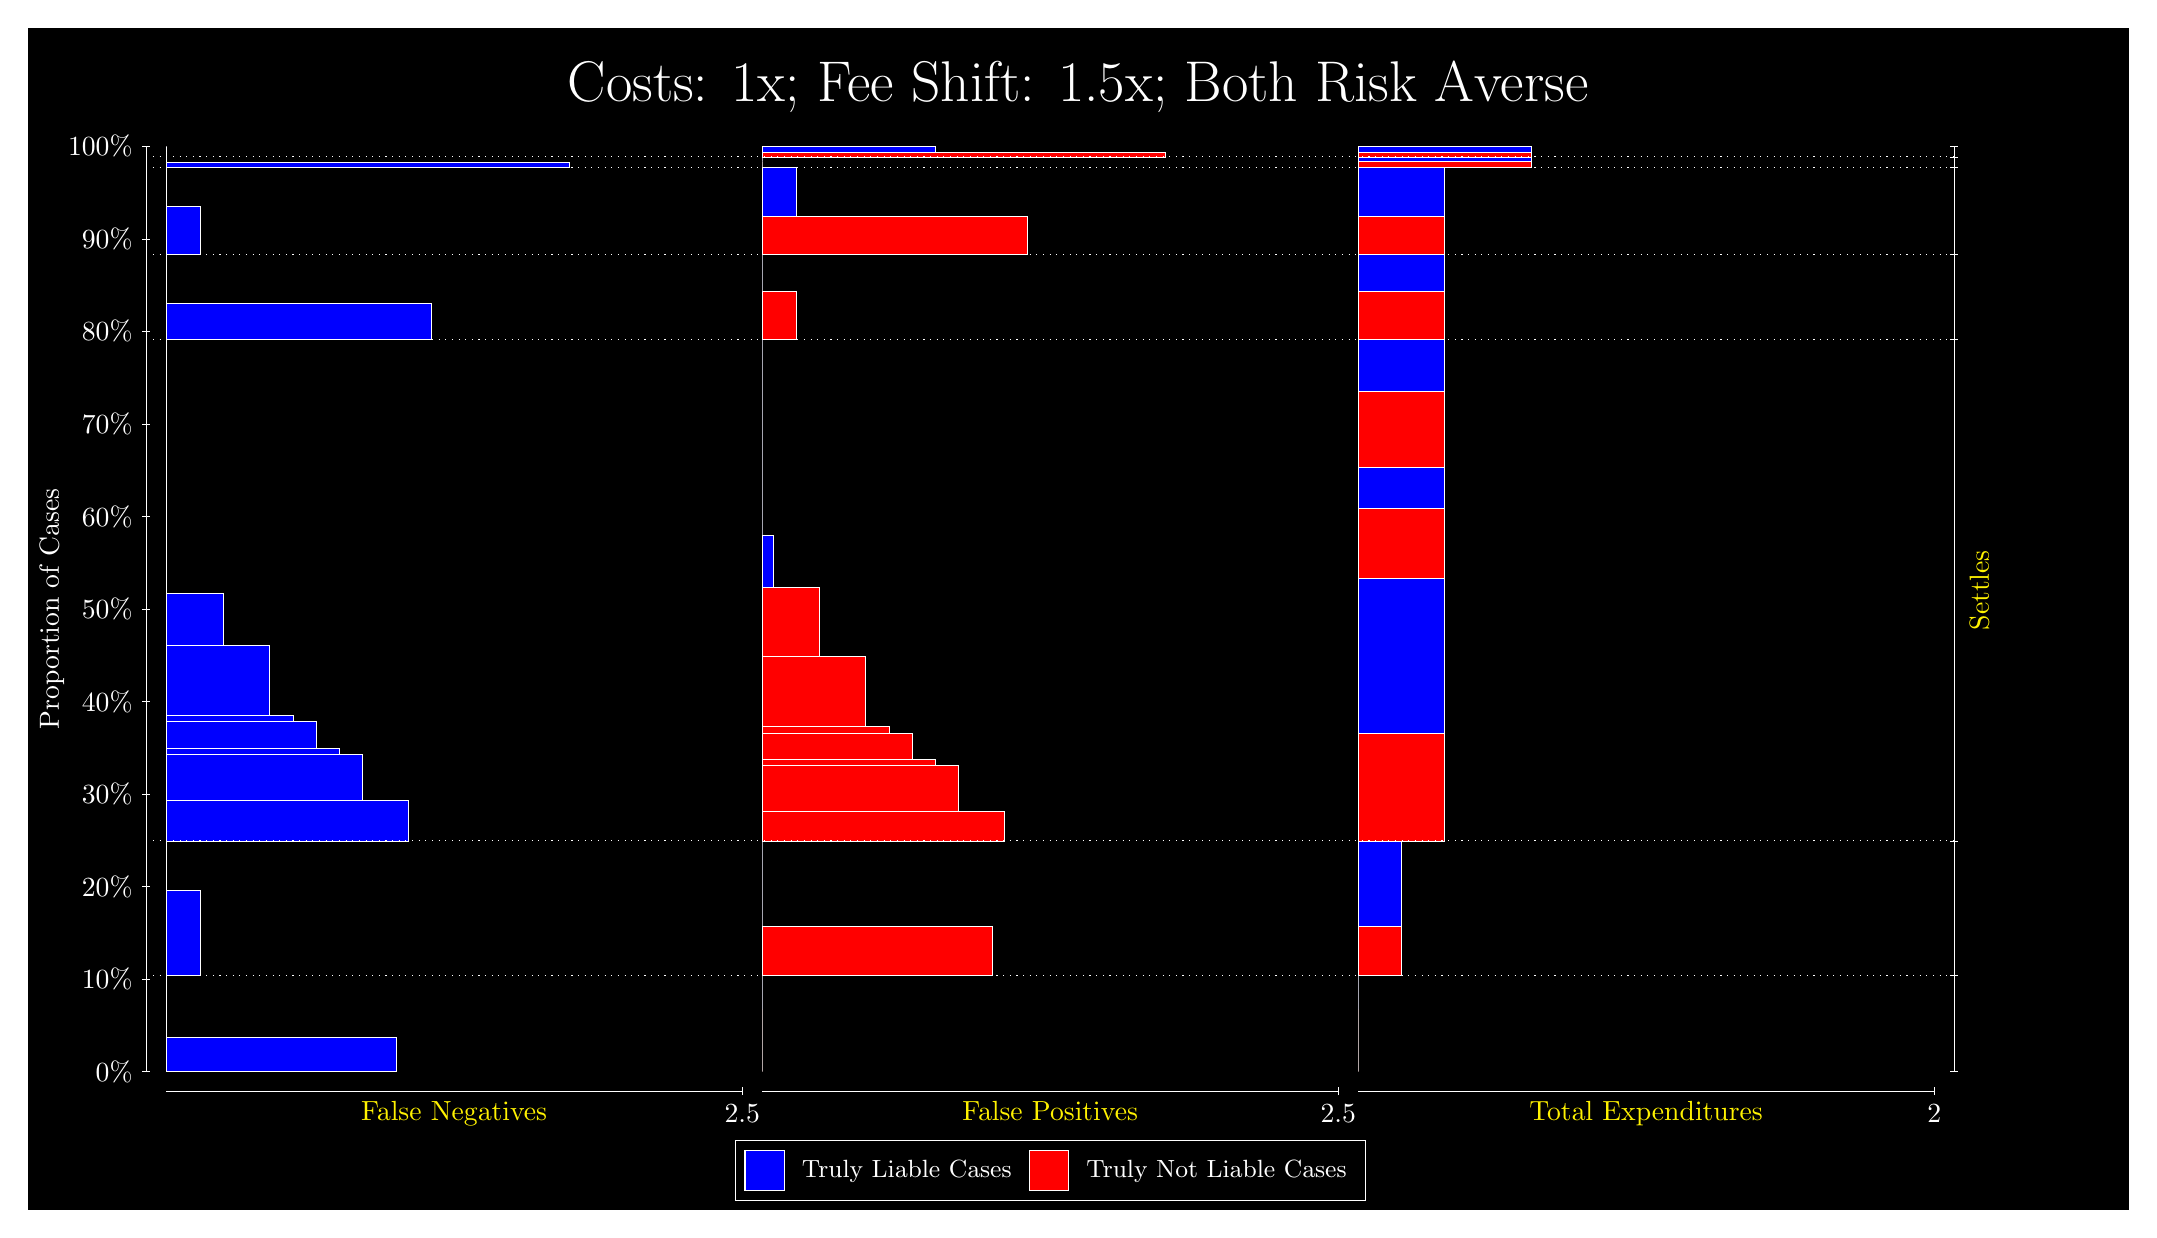
\begin{tikzpicture}
\draw[fill=black] (0,0) rectangle (26.667,15);
\draw[text=white] (0,13.5) rectangle (26.667,15) node[midway] {\huge Costs: 1x; Fee Shift: 1.5x; Both Risk Averse};
\draw[white, very thin] (1.5,1.75) -- (1.5,13.5);
\node[rotate=90, text=white, anchor=center] at (0.3, 7.625) {Proportion of Cases};
\draw[white, very thin] (1.45,1.75) -- (1.55,1.75);
\node[text=white, anchor=east] at (1.45, 1.75) {0\%};
\draw[white, very thin] (1.45,2.925) -- (1.55,2.925);
\node[text=white, anchor=east] at (1.45, 2.925) {10\%};
\draw[white, very thin] (1.45,4.1) -- (1.55,4.1);
\node[text=white, anchor=east] at (1.45, 4.1) {20\%};
\draw[white, very thin] (1.45,5.275) -- (1.55,5.275);
\node[text=white, anchor=east] at (1.45, 5.275) {30\%};
\draw[white, very thin] (1.45,6.45) -- (1.55,6.45);
\node[text=white, anchor=east] at (1.45, 6.45) {40\%};
\draw[white, very thin] (1.45,7.625) -- (1.55,7.625);
\node[text=white, anchor=east] at (1.45, 7.625) {50\%};
\draw[white, very thin] (1.45,8.8) -- (1.55,8.8);
\node[text=white, anchor=east] at (1.45, 8.8) {60\%};
\draw[white, very thin] (1.45,9.975) -- (1.55,9.975);
\node[text=white, anchor=east] at (1.45, 9.975) {70\%};
\draw[white, very thin] (1.45,11.15) -- (1.55,11.15);
\node[text=white, anchor=east] at (1.45, 11.15) {80\%};
\draw[white, very thin] (1.45,12.325) -- (1.55,12.325);
\node[text=white, anchor=east] at (1.45, 12.325) {90\%};
\draw[white, very thin] (1.45,13.5) -- (1.55,13.5);
\node[text=white, anchor=east] at (1.45, 13.5) {100\%};

\draw[white, very thin] (24.457,1.75) -- (24.457,13.5);
\draw[white, very thin] (24.407,1.75) -- (24.507,1.75);
\node[anchor=west] at (24.407, 1.75) {};
\draw[white, very thin] (24.407,2.9714) -- (24.507,2.9714);
\node[anchor=west] at (24.407, 2.9714) {};
\draw[white, very thin] (24.407,4.6795) -- (24.507,4.6795);
\node[anchor=west] at (24.407, 4.6795) {};
\draw[white, very thin] (24.407,11.045) -- (24.507,11.045);
\node[anchor=west] at (24.407, 11.045) {};
\draw[white, very thin] (24.407,12.123) -- (24.507,12.123);
\node[anchor=west] at (24.407, 12.123) {};
\draw[white, very thin] (24.407,13.232) -- (24.507,13.232);
\node[anchor=west] at (24.407, 13.232) {};
\draw[white, very thin] (24.407,13.367) -- (24.507,13.367);
\node[anchor=west] at (24.407, 13.367) {};
\draw[white, very thin] (24.407,13.5) -- (24.507,13.5);
\node[anchor=west] at (24.407, 13.5) {};

\draw[white, very thin, fill=blue] (1.75,1.75) rectangle (4.6775,2.1804);
\draw[white, very thin, fill=red] (1.75,2.1804) rectangle (1.75,2.9714);
\draw[white, very thin, fill=blue] (1.75,2.9714) rectangle (2.1891,4.0529);
\draw[white, very thin, fill=red] (1.75,4.0529) rectangle (1.75,4.6795);
\draw[white, very thin, fill=blue] (1.75,4.6795) rectangle (4.8239,5.2001);
\draw[white, very thin, fill=blue] (1.75,5.2001) rectangle (4.2384,5.7786);
\draw[white, very thin, fill=blue] (1.75,5.7786) rectangle (3.9457,5.8574);
\draw[white, very thin, fill=blue] (1.75,5.8574) rectangle (3.6529,6.1926);
\draw[white, very thin, fill=blue] (1.75,6.1926) rectangle (3.3602,6.2795);
\draw[white, very thin, fill=blue] (1.75,6.2795) rectangle (3.0674,7.1583);
\draw[white, very thin, fill=blue] (1.75,7.1583) rectangle (2.4819,7.8229);
\draw[white, very thin, fill=red] (1.75,7.8229) rectangle (1.75,11.045);
\draw[white, very thin, fill=blue] (1.75,11.045) rectangle (5.1167,11.512);
\draw[white, very thin, fill=red] (1.75,11.512) rectangle (1.75,12.123);
\draw[white, very thin, fill=blue] (1.75,12.123) rectangle (2.1891,12.742);
\draw[white, very thin, fill=red] (1.75,12.742) rectangle (1.75,13.232);
\draw[white, very thin, fill=blue] (1.75,13.232) rectangle (6.8732,13.292);
\draw[white, very thin, fill=red] (1.75,13.292) rectangle (1.75,13.367);
\draw[white, very thin, fill=red] (1.75,13.367) rectangle (1.75,13.427);
\draw[white, very thin, fill=blue] (1.75,13.427) rectangle (1.75,13.5);
\draw[white, very thin, fill=red] (9.3189,1.75) rectangle (9.3189,2.541);
\draw[white, very thin, fill=blue] (9.3189,2.541) rectangle (9.3189,2.9714);
\draw[white, very thin, fill=red] (9.3189,2.9714) rectangle (12.246,3.598);
\draw[white, very thin, fill=blue] (9.3189,3.598) rectangle (9.3189,4.6795);
\draw[white, very thin, fill=red] (9.3189,4.6795) rectangle (12.393,5.0593);
\draw[white, very thin, fill=red] (9.3189,5.0593) rectangle (11.807,5.6377);
\draw[white, very thin, fill=red] (9.3189,5.6377) rectangle (11.515,5.7165);
\draw[white, very thin, fill=red] (9.3189,5.7165) rectangle (11.222,6.0517);
\draw[white, very thin, fill=red] (9.3189,6.0517) rectangle (10.929,6.1386);
\draw[white, very thin, fill=red] (9.3189,6.1386) rectangle (10.636,7.0174);
\draw[white, very thin, fill=red] (9.3189,7.0174) rectangle (10.051,7.9015);
\draw[white, very thin, fill=blue] (9.3189,7.9015) rectangle (9.4652,8.5661);
\draw[white, very thin, fill=blue] (9.3189,8.5661) rectangle (9.3189,11.045);
\draw[white, very thin, fill=red] (9.3189,11.045) rectangle (9.758,11.656);
\draw[white, very thin, fill=blue] (9.3189,11.656) rectangle (9.3189,12.123);
\draw[white, very thin, fill=red] (9.3189,12.123) rectangle (12.686,12.613);
\draw[white, very thin, fill=blue] (9.3189,12.613) rectangle (9.758,13.232);
\draw[white, very thin, fill=red] (9.3189,13.232) rectangle (9.3189,13.306);
\draw[white, very thin, fill=blue] (9.3189,13.306) rectangle (9.3189,13.367);
\draw[white, very thin, fill=red] (9.3189,13.367) rectangle (14.442,13.427);
\draw[white, very thin, fill=blue] (9.3189,13.427) rectangle (11.515,13.5);
\draw[white, very thin, fill=red] (16.888,1.75) rectangle (16.888,2.541);
\draw[white, very thin, fill=blue] (16.888,2.541) rectangle (16.888,2.9714);
\draw[white, very thin, fill=red] (16.888,2.9714) rectangle (17.437,3.598);
\draw[white, very thin, fill=blue] (16.888,3.598) rectangle (17.437,4.6795);
\draw[white, very thin, fill=red] (16.888,4.6795) rectangle (17.986,6.0517);
\draw[white, very thin, fill=blue] (16.888,6.0517) rectangle (17.986,8.0171);
\draw[white, very thin, fill=red] (16.888,8.0171) rectangle (17.986,8.9012);
\draw[white, very thin, fill=blue] (16.888,8.9012) rectangle (17.986,9.4218);
\draw[white, very thin, fill=red] (16.888,9.4218) rectangle (17.986,10.388);
\draw[white, very thin, fill=blue] (16.888,10.388) rectangle (17.986,11.045);
\draw[white, very thin, fill=red] (16.888,11.045) rectangle (17.986,11.656);
\draw[white, very thin, fill=blue] (16.888,11.656) rectangle (17.986,12.123);
\draw[white, very thin, fill=red] (16.888,12.123) rectangle (17.986,12.613);
\draw[white, very thin, fill=blue] (16.888,12.613) rectangle (17.986,13.232);
\draw[white, very thin, fill=red] (16.888,13.232) rectangle (19.083,13.306);
\draw[white, very thin, fill=blue] (16.888,13.306) rectangle (19.083,13.367);
\draw[white, very thin, fill=red] (16.888,13.367) rectangle (19.083,13.427);
\draw[white, very thin, fill=blue] (16.888,13.427) rectangle (19.083,13.5);
\draw[white, dotted] (1.5,2.9714) -- (24.457,2.9714);
\draw[white, dotted] (1.5,4.6795) -- (24.457,4.6795);
\draw[white, dotted] (1.5,11.045) -- (24.457,11.045);
\draw[white, dotted] (1.5,12.123) -- (24.457,12.123);
\draw[white, dotted] (1.5,13.232) -- (24.457,13.232);
\draw[white, dotted] (1.5,13.367) -- (24.457,13.367);
\draw[white, very thin] (1.75,1.5) -- (9.0689,1.5);
\node[text=yellow, anchor=north] at (5.4094, 1.5) {False Negatives};
\draw[white, very thin] (9.0689,1.45) -- (9.0689,1.55);
\node[text=white, anchor=north] at (9.0689, 1.45) {2.5};

\draw[white, very thin] (9.3189,1.5) -- (16.638,1.5);
\node[text=yellow, anchor=north] at (12.978, 1.5) {False Positives};
\draw[white, very thin] (16.638,1.45) -- (16.638,1.55);
\node[text=white, anchor=north] at (16.638, 1.45) {2.5};

\draw[white, very thin] (16.888,1.5) -- (24.207,1.5);
\node[text=yellow, anchor=north] at (20.547, 1.5) {Total Expenditures};
\draw[white, very thin] (24.207,1.45) -- (24.207,1.55);
\node[text=white, anchor=north] at (24.207, 1.45) {2};



\node[text=yellow, centered, rotate=90] at (24.777, 7.8622) {Settles};





\draw (12.978300999999998,1.5) node[draw=none] (baseCoordinate) {};
\begin{scope}[align=center]
        \matrix[scale=0.5, draw=white, below=0.5cm of baseCoordinate, nodes={draw}, column sep=0.1cm]{
            \node[rectangle, draw, minimum width=0.5cm, minimum height=0.5cm, fill=blue] {}; &
            \node[draw=none, font=\small, text=white] (B) {Truly Liable Cases}; &
            \node[rectangle, draw, minimum width=0.5cm, minimum height=0.5cm, fill=red] {}; &
            \node[draw=none, font=\small, text=white] (B) {Truly Not Liable Cases}; \\
            };
\end{scope}

\end{tikzpicture}
\end{document}